\documentclass{article}
\usepackage{graphicx} % Required for inserting images
\usepackage{theoremstyle}
% \usepackage{amsthm}
% \usepackage{mdframed}
% \usepackage[most]{tcolorbox}
\usepackage{amsmath}
\usepackage{amsfonts}
\usepackage{enumerate}
\usepackage{blindtext}
\usepackage{enumitem}
\usepackage{float}
\usepackage{tikz}
\usetikzlibrary{calc}
\usepackage{varwidth}
\usepackage{bbm}
\usepackage{hyperref}
\hypersetup{
  colorlinks=true,
  linkcolor=blue,
  filecolor=magenta,
  urlcolor=PineGreen,
  pdftitle={Overleaf Example},
  pdfpagemode=FullScreen,
}
\usepackage[letterpaper, total={6.5in, 9in}]{geometry}
\usepackage[dvipsnames]{xcolor}

\urlstyle{same}
\title{Physics 1101W: Error Propagation}

\author{\color{SeaGreen} Sage Buesing}
\date{\today}
\newcommand{\Tr}{\text{Tr}}
\newcommand{\R}{{\mathbb R}}
\newcommand{\C}{{\mathbb C}}
\newcommand{\N}{{\mathbb N}}
\newcommand{\Z}{{\mathbb Z}}
\renewcommand{\L}{\mathcal{L}}
\newcommand{\Q}{{\mathbb Q}}
\newcommand{\sepline}{\break \vspace{0 cm} \hrulefill \vspace{0 cm} \break}
\newcommand{\B}{\mathcal{B}}
\newcommand{\integral}[2]{\int\limits_{#1}^{#2}}
\newcommand{\pder}[2]{\frac{\partial #1}{\partial #2}}
\renewcommand{\r}{\right}
\renewcommand{\l}{\left}
\renewcommand{\d}[1]{\text{d}#1}
\newcommand{\del}{\nabla}
\newcommand{\tder}[2]{\frac{\d{#1}}{\d{#2}}}
\newcommand{\n}{\newline}
\newcommand{\f}[2]{\frac{#1}{#2}}
\newcommand{\hb}{\hbar}
\newcommand{\paren}[1]{\left(#1\right)}
\renewcommand{\t}[1]{\text{#1}}


\begin{document}

\maketitle

Measurements that we make in the lab are not certain- a measurement depends on the fidelity of the instruments used.
This \textbf{Measurement Uncertainty}, and it is the most common form of \textbf{Random Error} or \textbf{Random Uncertainty}.


% \begin{center}
%   \fbox{
%     \begin{varwidth}{\linewidth}
%       \underline{\textbf{Note:}}\\
%       The words \textbf{Error} and \textbf{Uncertainty} are being pretty much used interchangeably here, and that will continue to largely be the case for this course.
%     \end{varwidth}
%   }
% \end{center}

\begin{note}
  The words \textbf{Error} and \textbf{Uncertainty} are being pretty much used interchangeably here, and that will continue to largely be the case for this course.
\end{note}

This is where you have to worry about propagating error, because when we \emph{use} measurements from our experiment to find a \textbf{Derived Quantity}, we want to know how certain (or not) we are about that value. For a more formal treatment of addition of randomly distributed measurements see\footnote{\url{https://en.wikipedia.org/wiki/Sum_of_normally_distributed_random_variables}}. Such treatments will \textbf{NOT} be used in this class, and our treatment is far less rigorous than the above.


\begin{definition}[Derived Quantity]
  A \textbf{Derived Quantity} is a value of a property of a system that is not being directly measured. A \textbf{Derived Quantity} is found from quantities that we \emph{did} measure directly.
\end{definition}

Let's quickly go over the anatomy of a measurement. Measurements are composed of a \textbf{Central Value} and a \textbf{Variance}.

\begin{definition}[Central Value \emph{or} Mean]
  The \textbf{Central Value}(or the \textbf{Mean}) of a measurement is the main number we usually think of as a measurement's output- basically it's what the instrument reads. If I were to measure a mass to be $71$g, that is the central value.
\end{definition}

It is worth noting (by the conceit of measurement uncertainty) that when we measure a central value, that is not a completely accurate representation of that quantity as a whole. Due to random noise, all sorts of general errors that might occur in the measurement process, instrument calibration process, etc., we can assume that our measurements are reasonably close to the \emph{actual} value. Mathematically, we can think of this spread as a \emph{\href{https://en.wikipedia.org/wiki/Normal\_distribution}{normal distribution}}. All you need to consider for this class is the idea that the \textbf{Central Value} is the most likely value for the ``actual" value to be, but with decreasing likelyhood as we drift further from that center, there is a range that the ``actual" value can fall within.

\begin{figure}
  \centering
  \includegraphics[width=0.7\linewidth]{assets/Uniform.png}
  \caption{
    \textbf{Measurement Distributions}
    The measured central value $m$ with respect to two types of measurement distribution. We see that the variance $\delta m$ is (half) the width of our uniform distribution, and is equal to (half) the width between the points where the probability is $\frac{1}{e}$ times the maximum probability for the normal distribution.
  }
  \label{fig:dist}
\end{figure}


\begin{definition}[Variance]
  For our purposes, instead of a normal distribution, we are treating our measurements more like a box where our variance is half of the width of the box. This represents the range of possible values around our central value that we are considering as possible ``actual" values for a measurement.
\end{definition}

The goal of error propagation is thus to find the error in a Derived Quantity from the error in the measurements we're using to \emph{find} that quantity. To do so, we have to use some combination of 3 fundamental equations.

\begin{lemma}[Error Propagation]
  In the statement below, let us use capital letters for quantities with uncertainties, and lower case letters for constant/scalar values (things like fundamental constants- think of just normal numbers such as $2, 9.81$ or $\pi = 3.1415\ldots$)
  \begin{align}
    \delta \left(c*A\right) &= c*\delta A \label{eq:scalar}\\
    \delta\left(A+B\right) &= \delta A + \delta B \label{eq:add}\\
    \delta\left(A * B\right) &= \left(A*B\right)\left(\frac{\delta A}{A} + \frac{\delta B}{B}\right)\label{eq:mult}
  \end{align}
\end{lemma}

\begin{note}
  We can use the same equation for $A-B$ as for $A+B$, and similarly the same equation for $\frac{A}{B}$ as for $A*B$.
\end{note}

Note also that these equations can be combined/chained. By this, I mean that an uncertainty that we found by applying one of the above quantities can be used again in further error/uncertainty propagation equations.

Let's use an example

\begin{example}
  \label{ex:scalar}
  Consider two masses $m_1$ and $m_2$. We can measure each of these masses on our balance. Take $m_1$ to be the full mass hanger that we use in labs (hook etc. included), and $m_2$ to be one of the $20 g$ weight disks.

  Say we hang $m_2$ on the $m_1$ hanger, and weigh them both together on a balance, which reads $71 \mathrm{g}$. Call this mass of the combined hanger and disk $m_s$.

  If we take for given that the uncertainty we get from massing a sample on our balance is $\pm 5\mathrm{g}$, what should you provide in your lab report as the weight ($W_s$) of these two masses together when hung from a spring during an experiment?

  \medskip
  \hrule
  \medskip

  \textbf{Answer:}

  We can find the uncertainty in $W_s$ using Equation \eqref{eq:scalar}.

  \begin{align}
    \intertext{First finding our derived quantity's central value}
    W_s &= (m_s)\mathrm{g} = 71 \mathrm{g} * 9.81 \frac{\mathrm{m}}{\mathrm{s}^2} = 0.071 \mathrm{kg} * 9.81 \frac{\mathrm{m}}{\mathrm{s}^2}\notag\\
    &= 0.69651 \frac{kg*m}{s^2} = 0.70\mathrm{N} \text{(up to sig figs)}\notag
    \intertext{Applying equation Equation \eqref{eq:scalar}, where $m_s$ is our measured quantity (with uncertainty) and $g$ is our scalar, and plugging in $m_s \rightarrow A, \quad g \rightarrow c$}
    \delta W_s &= g * \delta m_s \label{eq:scaapp} \\
    \delta W_s &= 9.81 \frac{\mathrm{m}}{\mathrm{s}^2} * 5 \mathrm{ g} = 9.81 \frac{\mathrm{m}}{\mathrm{s}^2} * 0.005 \mathrm{ kg}\notag\\
    &= 0.04905 \frac{\mathrm{kg*m}}{\mathrm{s^2}} = 0.049 \mathrm{N}
  \end{align}

  Thus we would report a full measurement of our weight $W_s$ as $W_s = 0.70 \pm 0.049 \mathrm{N}$.


\end{example}

One thing to be aware of here is that we are somewhat abusing notation: we used $W_s$ above sometimes to refer to the Central Value of the measurement, and other times to refer to the measurement as a whole, including uncertainty. This is another bit of terminology you will have to get used to somewhat, unless you want to introduce even more subscripts! As a general rule, if you have doubts report quantities \emph{with} uncertainties.

\begin{example}
  Now consider if we were to measure each mass separately: $m_1$ being measured by the balance as $51 \mathrm{g}$ and $m_2$ at $24 \mathrm{g}$

  \medskip
  \hrule
  \medskip

  \textbf{Answer:}

  Measuring both of these quantities separately means that both $m_1$ and $m_2$ will carry uncertainty.

  The total mass hanging from the spring can be expressed as

  \begin{equation}
    m_s = m_1 + m_2
  \end{equation}

  First we can find the central value of $m_s$ just by normal addition

  \begin{equation}
    m_s = 51 \mathrm{g} + 24 \mathrm{g} = 75 \mathrm{g}\notag
  \end{equation}

  Which gives $W_s=0.075\mathrm{kg}*9.81 \frac{\mathrm{m}}{\mathrm{s}^2} = 0.73 \mathrm{N}$

  We can find the uncertainty in $m_s$ using Equation \eqref{eq:add}.  Consider substituting in $m_1 \rightarrow A$ and $m_2 \rightarrow B$.

  \begin{align}
    \delta\left(m_s\right) &= \delta\left(m_1 + m_2\right) = \delta m_1 + \delta m_2\\
    &= 5 \mathrm{g} + 5 \mathrm{g}\notag\\
    &= 10 \mathrm{g}\notag
  \end{align}

  Now to find the uncertainty in weight, we want $\delta\left(W_s\right) = \delta\left(m_sg\right)$

  Plug this back into Equation \eqref{eq:scalar} like we did in Equation \eqref{eq:scaapp} to find

  \begin{align}
    \delta\left(W_s\right)&=\delta\left(m_sg\right) = g*\delta m_s\notag\\
    &=9.81 \frac{\mathrm{m}}{\mathrm{s}^2} * 10 \mathrm{g} = 9.81 \frac{\mathrm{m}}{\mathrm{s}^2} * 0.01 \mathrm{kg}\notag\\
    &=0.091 \mathrm{N}
  \end{align}

  And thus we would report $W_s = 0.73 \pm 0.091 \mathrm{g}$

  It is somewhat satisfying to note that $0.73 \mathrm{N}$ is in fact within both of our uncertainties of the Central Value we found in Example \ref{ex:scalar}! This must be the case though, since we propagated our errors correctly, the fact that Central Value we found at the start of this example is still within the uncertainty we had when measuring both masses together in Example \ref{ex:scalar} assures us that this is a possible outcome of measuring the two masses separately after measuring them together. Thus these calculations should be consistent.
\end{example}

As was said before, we will use many of these equations in sequence. Finally, let's practice a bit more complicated situation.

\newpage
\begin{example}
  Consider a block sliding on a horizontal surface without friction, being pulled by a hanging block on a string. The hanging block is hanging vertically off the surface, with the string connecting them over a frictionless pulley.

  Find the acceleration experienced by Block 1.
  \begin{figure}[H]
    \centering
    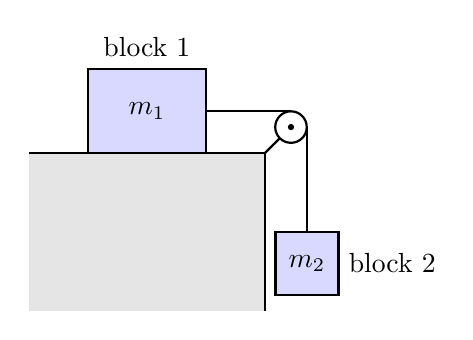
\begin{tikzpicture}[thick, scale=1]

      % horizontal ledge
      \fill[gray!20] (-0,0) rectangle (3,-2);
      \draw (0,0) -- (3,0);
      \draw (3,0) -- (3,-2);
      % \draw (0,0) -- (4,0);
      % \foreach \x in {-0.4,-0.1,...,4.8}
      % \draw (\x,0) -- ++(-0.5,-0.5);

      % pulley
      \coordinate (p) at (3.33,0.33);
      \draw (p) circle (0.2);
      \fill (p) circle (0.04);

      % block on ledge
      \draw[fill=blue!15] (0.75,0) rectangle (2.25,2*.5333);
      \node at (1.5,.5333) {$m_1$};

      % hanging block
      \draw[fill=blue!15] (3.5333-0.4,-1) rectangle (3.5333+0.4,-1.8);
      \node at (3.5333,-1.4) {$m_2$};

      % string
      \draw (2.25,.5333) -- (3.33,.5333);
      \draw (3.5333,.333) -- (3.5333,-1);
      % -- (4,0.65);

      %rod
      \draw (3,0) -- (3.1919,0.1919);

      % labels
      \node[above] at (1.5,1.1) {block 1};
      \node[right] at (3.5333+0.4,-1.4) {block 2};

    \end{tikzpicture}
  \end{figure}

  \medskip
  \hrule
  \medskip

  \textbf{Answer:}

  From a simple application of Newton's second law, we know that the acceleration of Block 1 should be (with the positive $x$ axis pointing to the right
    \begin{equation}
      a_1=g*\frac{m_2}{m_1+m_2}\label{eq:blockq}
    \end{equation}

    From this we can see that we will need to apply all three of the Error Propagation equations to find the uncertainty in the acceleration.

    Let's work from the inside out, and as a good exercise let's make sure \emph{not} to plug in any numbers until the end- it makes keeping track of sig figs, approximations, and just page clutter easier overall.

    \begin{equation}
      \delta(m_1+m_2) = \delta m_1 + \delta m_2\notag
    \end{equation}

    From here we can note that this uncertainty can be plugged into the uncertainty for multiplication and division (Equation \eqref{eq:mult}) with $m_2 \rightarrow A, \left(m_1+m_2\right) \rightarrow B$.

    \begin{align}
      \delta\left(\frac{m_2}{m_1+m_2}\right)&=\frac{m_2}{m_1+m_2}\left(\frac{\delta m_2}{m_2} + \frac{\delta \left(m_1 + m_2\right)}{m_1+m_2}\right)\notag\\
      &=\frac{m_2}{m_1+m_2}\left(\frac{\delta m_2}{m_2} + \frac{\delta m_1 + \delta m_2}{m_1+m_2}\right)\label{eq:blockm}
    \end{align}

    Finally, we can use Equation \eqref{eq:scalar} to tell us that

    \begin{equation}
      \delta\left(g\left(\frac{m_2}{m_1+m_2}\right)\right)=g*\delta\left(\frac{m_2}{m_1+m_2}\right)
    \end{equation}
    Using Equation \eqref{eq:blockm} gives us

    \begin{equation}
      \delta a_1 = \delta\left(g\frac{m_2}{m_1+m_2}\right) =g\left(\frac{m_2}{m_1+m_2}\right)\left(\frac{\delta m_2}{m_2} + \frac{\delta m_1 + \delta m_2}{m_1+m_2}\right)\label{eq:blounc}
    \end{equation}

  \end{example}
  \begin{example}[Answer cont.]

    For simplicity, take the values of $m_1$ and $m_2$ that we had before, with $5 \mathrm{g}$ uncertainty. First, finding the Central Value (Equation \eqref{eq:blockq}):

    \begin{align}
      a_1&=g\frac{m_2}{m_1+m_2}\\
      &=9.81 \frac{\mathrm{m}}{\mathrm{s}^2} *  \frac{24 \mathrm{g}}{51 \mathrm{g} + 24 \mathrm{g}}\\
      \intertext{The units of mass cancel and we get}
      &= 9.81 \frac{\mathrm{m}}{\mathrm{s}^2} * 0.32\\
      &= 3.1\frac{\mathrm{m}}{\mathrm{s}^2} \text{ (up to sig figs)}
    \end{align}

    Now for uncertainty. Using Equation \eqref{eq:blounc}

    \begin{align}
      \delta a_1 &=  9.81 \frac{\mathrm{m}}{\mathrm{s}^2}\left(\frac{24 \mathrm{g}}{51 \mathrm{g}+24 \mathrm{g}}\right)\left(\frac{5 \mathrm{g}}{24 \mathrm{g}} + \frac{ 5 \mathrm{g} + 5 \mathrm{g}}{51 \mathrm{g} + 24 \mathrm{g}}\right)\\
      \intertext{Again, units of mass cancel}
      &= 9.81 \frac{\mathrm{m}}{\mathrm{s}^2} * \frac{24}{75}\left(\frac{5}{24} + \frac{10}{75}\right)\\
      &\approx 1.1  \frac{\mathrm{m}}{\mathrm{s}^2}
    \end{align}
    Thus we would report $a_1 = 3.1 \pm 1.1\frac{\mathrm{m}}{\mathrm{s}^2}$
  \end{example}

  That's a pretty large uncertainty! As you can see, uncertainties can compound to become quite important, even if they seem somewhat inconsequential at first.

  \end{document}
